\newcolumntype{C}{>{\centering\arraybackslash}m{.12\linewidth}}
\newcolumntype{Y}{>{\centering\arraybackslash}X}

\begin{table*}
    \normalsize\medskip\noindent
    \begin{tabularx}{\textwidth}{l| *{6}{Y}}
        \toprule \multicolumn{7}{l}{{\underline{\textbf{\textsc{Entrées}}}}}
        \\ &
        \multicolumn{1}{Y}{\includegraphics{tikz/compass}} &
        \multicolumn{1}{Y}{\includegraphics{tikz/knees}} &
        \multicolumn{2}{c}{\includegraphics{tikz/compass_bust}} &
        \includegraphics{tikz/compass_neck} &
        \includegraphics{tikz/arms}
        \\ Modèle & $M_A$ & $M_B$ & \multicolumn{2}{c}{$M_C$} & $M_D$ & $M_E$
        \\ Description & Compas & $M_A$ avec des genous &
        \multicolumn{2}{c}{$M_A$ avec un buste} &
        \multicolumn{1}{Y}{$M_C$ avec un cou} &
        \multicolumn{1}{Y}{$M_C$ avec des bras}
        \\  \rowcolor{gray!20}
        Masse totale & 33.1\,kg & 33.1\,kg & 60.3\,kg & 60.3\,kg & 60.3\,kg & 65.9\,kg
        \\ Actionnement & actif & actif & actif & \textbf{passif} & actif & actif
        \\  \rowcolor{gray!20}
        Dimension & 2D & 2D & 2D & 2D & 2D & \textbf{3D}
        \\ \midrule \multicolumn{7}{l}{{\underline{\textbf{\textsc{Sorties}}}}}
        \\ &
        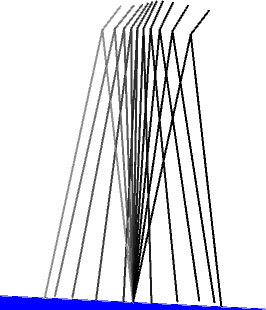
\includegraphics[height=4cm]{imgs/2_100_fixed.png} &
        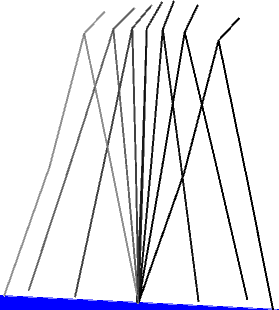
\includegraphics[height=4cm]{imgs/2_100_fixed_kneeled.png} &
        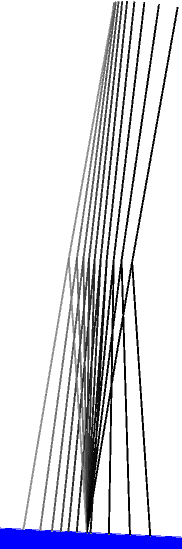
\includegraphics[height=4cm]{imgs/2_100_fixed_with_bust.png} &
        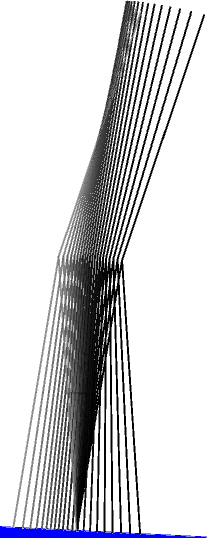
\includegraphics[height=4cm]{imgs/2_100_fixed_passive.png} &
        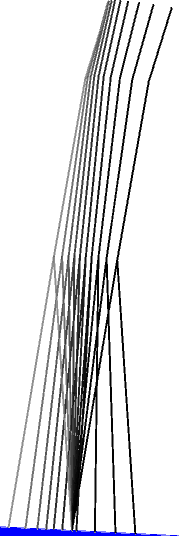
\includegraphics[height=4cm]{imgs/2_100_fixed_with_neck.png} &
        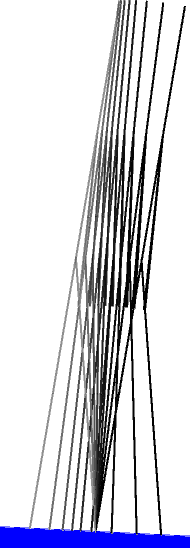
\includegraphics[height=4cm]{imgs/2_100_fixed_3d.png}
        \\ \rowcolor{gray!20}
        CoT & 0.1007 & 0.0544 & 0.0618 & 0.0499 & 0.0621 & 0.0651
        \\ Longueur & 0.56\,m & 0.85\,m & 0.40\,m & 0.40\,m & 0.40\,m & 0.41\,m
        \\ \rowcolor{gray!20}
        Vitesse &  0.70\,m/s & 1.06\,m/s & 0.50\,m/s & 0.50\,m/s & 0.50\,m/s & 0.51\,m/s
        \\ \midrule \multicolumn{7}{l}{{\underline{\textbf{\textsc{Performances}}}}}
        \\ Itérations & 56 & 40 & 76 & 9 & 66 & 108
        \\ \rowcolor{gray!20}
        Durée & 2.8\,s & 2.9\,s & 2.6\,s & 1.2\,s & 4.1\,s & 7.6\,s
        \\ \bottomrule
    \end{tabularx}
    \caption{Six marcheurs bipèdes sont comparés afin de déterminer l'influence des genous, du buste, du cou, des bras,
    et du type d'actionnement. Pour chaque exemple, l'algorithme nous fourni la démarche, le coût final de transport
    optimisé et la longueur d'un pas. Les deux dernières lignes donnent les performances de l'algorithme. Dans tous ces
    exemples, la durée d'un pas est fixée à 0.8 secondes et la pente du sol à 0.05 radians.}
    \label{tbl:results}
\end{table*}
